\section{Limitation of Previous Models}
\label{sec:non_linear}

Since directly measuring the power draw of every pixel color is too
costly (\eg it would take $256^3$$\times$10 seconds or 5.3 years following
our methodology), power modeling has been proposed to estimate the OLED
power draw of any pixel color based on measurements of a few pixel colors.

% additive model
% linear regression
% non-linear modeling

% Linear (r+g+b)
% linear (*r + *g + * b +(r+g+b)) 
% Kim is some hack - cannot reproduce

\paragraph{Simple linear model.}
\label{subsec:LM}
Dong~\etal~\cite{dong2009current} proposed one of the first pixel-level OLED current models,
which models the pixel power draw as the simple sum of
those of subpixels:
\begin{equation}
	P_i(R_i, G_i,B_i) = f(R_{i}) + g(G_{i}) + h(B_{i})
	\label{eq:linear_equation}
\end{equation}
and showed that the model  achieves an average 
error of 1\% in
displaying 300 benchmark images on an external OLED QVGA display
module with a standard 16-bit (5, 6, 5) RGB setting.
%
The simple linear model (denoted as LM) cannot model the OLED power on modern phones
which violate the superposition property.
%as discussed in \S\ref{subsec:super}.

%   We note the model of interest in this paper
%   is that of the pixel power draw as a function of the power
%   draw of subpixels, which we denote this as {\em pixel power model}.
%   The individual subpixel power draw 
%   $f(R_{i})$, $g(G_{i}$, and $h(B_{i})$ are known to be linear with respect to
%   the color value $R_{i}, G_i, B_i$ after gamma correction~\cite{???}.

%  The above property pertains to power behavior of subpixels within a pixel.
%  Since the individual subpixel power draw functions
%  $f(R_{i})$, $g(G_{i}$, and $h(B_{i})$ are known to be monotonically increasing with respect to
%  the color values $R_{i}, G_i, B_i$~\cite{???}, any linear pixel power model
%  also posses the following property:

%  \begin{itemize}
%  \item {\bf Monotonicity:} The higher the RGB values, the higher the pixel power draw.
%    For example, RGB values of (32, 32, 32) will result in higher pixel power draw than
%    RGB values of (32, 32, 0).
%  \end{itemize}


\paragraph{Adding Linear Regression.}
\label{subsec:LMLR}
Violation of the superposition property has been observed
previously~\cite{mittal2012empowering,kim2013runtime}
and suggests the power draw of three subpixels
are not independent.
The simplest idea to accommodate the dependence is to introduce liner regression,
as suggested by Kim~\etal~\cite{kim2013runtime},
%  performed one of the first
%  validations of the simple OLED power model (Eqn.~\ref{eq:linear_equation}
%  on smartphones and also
\forjnl{, who were among the first to discover that the OLED power draw violates the
  superposition property.}
who showed extending the
simple summation into a linear formula with the coefficients dervied
via linear regression reduces the average error from 8.0\% to 1.4\% on
Galaxy S3 for a set of screen images of 10 Android apps.

\if 0
\begin{equation}
P_i = Br\cdot(f(R_{i}) + g(G_{i}) + h(B_{i}) + e(R_{i},G_{i},B_{i}))
\label{eq:linear_equation2}
\end{equation}
\noindent
where $Br$ is the normalized brightness level and $e(R,G,B)= a(R+G+B)
+ b$, is a linear regression term with empirically estimated
coefficients. \
\fi

\if 0
To validate if linear regression can capture the OLED power behavior
on the 3 modern phones in our experiments, we derive linear
regressions on the power draw of the 3 base colors to fit the power
draw of the 3 2-channel colors (yellow, magenta and cyan) and 1 3-channel color (white).
Eqn.~\ref{eq:linear_independent} shows the coefficients of the linear
regressions.  We see that the coefficients of the four linear
regressions differ significantly, suggesting the dependence among the
power draw of subpixel cannot be easily captured with a single linear
model from linear regression.

\begin{subequations}
\begin{align}
	&\begin{bmatrix}
	    P_{y} \\
	    P_{m} \\
	    P_{c} \\
	    P_{w}
	\end{bmatrix}
	=
	\begin{bmatrix}
		T
	\end{bmatrix}
	\begin{bmatrix}
	    P_{r} &
	    P_{g} &
	    P_{b}
	\end{bmatrix}^T
	\\
	&\begin{bmatrix}
		T
	\end{bmatrix}
	=
	\mbox{Coefficients from linear regression to fit 4 colors} \nonumber
	\\
	&Nexus 6: \nonumber
	\\
	&\begin{bmatrix}
	     1.091 &      0.607 &      0.000 \\
	     1.539 &      0.000 &      0.015 \\
	     0.000 &      1.982 &      0.244 \\
	     0.621 &      1.586 &      0.029
	\end{bmatrix}
	\\
	&Moto Z3:  \nonumber
	\\
	&\begin{bmatrix}
	     1.103 &      0.439 &      0.000 \\
	     0.247 &      0.000 &      1.226 \\
	     0.000 &      0.023 &      1.338 \\
	     0.942 &      0.693 &      0.327
	\end{bmatrix}
	\\
	&Pixel 2:  \nonumber
	\\
	&\begin{bmatrix}
	     0.544 &      1.489 &      0.000 \\
	     0.638 &      0.000 &      1.000 \\
	     0.000 &      1.193 &      0.739 \\
	    -0.201 &      4.125 &     -0.401
	\end{bmatrix}
\end{align}
	\label{eq:linear_independent}
\end{subequations}
\fi

\forjnl{Figure~\ref{fig:initial_evaluation_2} shows that the
OLED display power for based colors red, green, and blue ($f(R_{i})$,
$g(G_{i})$, and $h(B_{i})$) and white and magenta are all linear w.r.t.
the linear RGB value.  Therefore, it is conceivable to derive a linear
regression of $f(R_{i})$, $g(G_{i})$, and $h(B_{i})$ to match well with
the OLED power draw of any single color, \eg white.
}

Since the power model should model the pixel power draw for
any combinations of RGB values, to assess the feasibility of the above model, we 
derived linear regression of $f(R_{i})$, $g(G_{i})$, and $h(B_{i})$ 
to fit the power draw of 4 colors, yellow, magenta and cyan, and white,
as the intensity varies from 0 to 255\footnote{We use 4-color monochromatic images to train these
  models because that they cover the sRGB space and gives us 256$\times$4=1024 equations.
  Training the models using real images may not cover the entire color space or provide
  enough diversity.}. The derived models
for the 3 phones are:

\hspace{-0.1in}
{\small
  \begin{eqnarray}
%\begin{align}
	P_i^{Pixel 2} = 0.700*f(R_i) + 0.928*g(G_i) + 0.868*h(B_i) \\
	P_i^{Moto Z3} = 0.665*f(R_i) + 0.928*g(G_i) + 0.708*h(B_i) \\
	P_i^{Pixel 4} = 0.779*f(R_i) + 1.047*g(G_i) + 0.929*h(B_i)
%\end{align}
	\label{eq:linear_model_linear_regression}
  \end{eqnarray}
}
\noindent
The models do not have constant terms because the base power is
already accounted in Eqn.~\ref{eq:linear_equation0}.

We then plot the predicted power with the new models for magenta and white in
Figure~\ref{fig:initial_evaluation_2}, labeled as LMLR.  We see that the new model
improves the accuracy of the simple superposition model LM, but still
incurs an average (over linear RGB values)
prediction error of 13\%, 9\%, and 8\% for white
and 13\%, 14\%, and 7\% for magenta (not shown) on the 3 phones, respectively.

A second reason that such linear regression based models are inaccurate
is that they are linear in the subpixel powers (with positive coefficients), and hence still
assume the monotonicity property which does not hold as shown
in \S\ref{subsec:monoproperty}.

% \begin{equation}
% 	\begin{bmatrix}
% 	    y \\
% 	    m \\
% 	    c \\
% 	    w
% 	\end{bmatrix}
% 	=
% 	\begin{bmatrix}
% 	     1.091 &      0.607 &      0.000 \\
% 	     1.539 &      0.000 &      0.015 \\
% 	     0.000 &      1.982 &      0.244 \\
% 	     0.621 &      1.586 &      0.029
% 	\end{bmatrix}
% 	\begin{bmatrix}
% 	    r \\
% 	    g \\
% 	    b
% 	\end{bmatrix}
% 	\label{eq:linear_independent}
% \end{equation}
% 
% \begin{equation}
% 	\begin{bmatrix}
% 	    y \\
% 	    m \\
% 	    c \\
% 	    w
% 	\end{bmatrix}
% 	=
% 	\begin{bmatrix}
% 	     1.103 &      0.439 &      0.000 \\
% 	     0.247 &      0.000 &      1.226 \\
% 	     0.000 &      0.023 &      1.338 \\
% 	     0.942 &      0.693 &      0.327
% 	\end{bmatrix}
% 	\begin{bmatrix}
% 	    r \\
% 	    g \\
% 	    b
% 	\end{bmatrix}
% \end{equation}
% 
% \begin{equation}
% 	\begin{bmatrix}
% 	    y \\
% 	    m \\
% 	    c \\
% 	    w
% 	\end{bmatrix}
% 	=
% 	\begin{bmatrix}
% 	     0.544 &      1.489 &      0.000 \\
% 	     0.638 &      0.000 &      1.000 \\
% 	     0.000 &      1.193 &      0.739 \\
% 	    -0.201 &      4.125 &     -0.401
% 	\end{bmatrix}
% 	\begin{bmatrix}
% 	    r \\
% 	    g \\
% 	    b
% 	\end{bmatrix}
% \end{equation}


\paragraph{Using non-linear models.}
\label{subsec:nonlinear}
Another measurement study~\cite{park2015accurate} on an external
AMOLED module
% also
suggested % subpixels are not independent and proposed
adding non-linear terms, in particular, pairwise two-color
coupling terms, to reduce the modeling error of linear models.


\if 0
Eqn.\ref{eq:linear_dependent} the resulting coefficients.

\begin{subequations}
\begin{align}
	&\begin{bmatrix}
	    P_{y} \\
	    P_{m} \\
	    P_{c} \\
	    P_{w}
	\end{bmatrix}
	=
	\begin{bmatrix}
		T
	\end{bmatrix}
	\begin{bmatrix}
	    P_{r} 	       &
	    P_{g} 	       &
	    P_{b} 	       &
	    P_{r}*P_{g}        &
	    P_{r}*P_{b}        &
	    P_{b}*P_{g}        &
	    P_{r}*P_{g}*P_{b}
	\end{bmatrix}^T
	\\
	&\begin{bmatrix}
		T
	\end{bmatrix}
	=
		Linear Dependent Transformation \nonumber
	\\
	&Nexus 6: \nonumber
	\\
	&\begin{bmatrix}
	      1.11 &       0.57 &       0.00 &       0.00 &       0.00 &       0.00 &       0.00 \\
	      1.20 &       0.00 &      -0.16 &       0.00 &       0.00 &       0.00 &       0.00 \\
	      0.00 &       2.70 &       0.21 &       0.00 &       0.00 &      -0.00 &       0.00 \\
	      1.37 &       1.97 &      -1.53 &      -0.04 &       0.03 &       0.00 &      -0.00
	\end{bmatrix}
	\\
	&Moto Z3: \nonumber
	\\
	&\begin{bmatrix}
	      1.14 &       0.18 &       0.00 &       0.00 &       0.00 &       0.00 &       0.00 \\
	     -0.41 &       0.00 &       1.27 &       0.00 &       0.00 &       0.00 &       0.00 \\
	      0.00 &      -0.17 &       1.37 &       0.00 &       0.00 &       0.00 &       0.00 \\
	      0.98 &       2.34 &      -1.07 &      -0.04 &       0.01 &       0.02 &       0.00
	\end{bmatrix}
	\\
	&Pixel 2: \nonumber
	\\
	&\begin{bmatrix}
	      0.64 &       1.29 &       0.00 &       0.00 &       0.00 &       0.00 &       0.00 \\
	     -0.04 &       0.00 &       1.12 &       0.00 &       0.01 &       0.00 &       0.00 \\
	      0.00 &       1.76 &       0.49 &       0.00 &       0.00 &      -0.00 &       0.00 \\
	     -1.41 &       3.25 &       0.34 &      -0.13 &       0.09 &      -0.02 &       0.00
	\end{bmatrix}
\end{align}
	\label{eq:linear_dependent}
\end{subequations}
\fi

  \if 0
  &\begin{bmatrix}
	    P_{y} \\
	    P_{m} \\
	    P_{c} \\
	    P_{w}
	\end{bmatrix}
  \fi

We experimented with such a non-linear model (denoted as NLM),
by adding pairwise two-color
coupling terms and a three-color coupling term,
and applying linear regression to derive the coefficients
of the resulting polynomial model to fit the power draw
of the same 4 colors, yellow, magenta and cyan, and white:

\hspace{-0.2in}
  {\small
  \begin{eqnarray}
  P&=&V\cdot [ 
	    f(Ri)\mbox{\hspace{0.07in}}
	    g(G_i)\mbox{\hspace{0.07in}}
	    h(B_i)\mbox{\hspace{0.07in}}
	    f(Ri)\cdot g(G_i)\mbox{\hspace{0.07in}}\\
&&	    f(Ri)\cdot h(B_i)\mbox{\hspace{0.07in}}
	    g(G_i)\cdot h(B_i)\mbox{\hspace{0.07in}}
	    f(Ri)\cdot g(G_i)\cdot h(B_i)
  ]^T
	\nonumber \\
%V=	\mbox{Coefficients from linear regression to fit 4 colors} \nonumber \\
        V_{Pixel 2} &=& \lbrack 0.33\mbox{\hspace{0.07in}}
        0.61\mbox{\hspace{0.07in}}
        0.65\mbox{\hspace{0.07in}}
        0.01\mbox{\hspace{0.07in}}
        0.01\mbox{\hspace{0.07in}}
        0.01\mbox{\hspace{0.07in}}
        -0.00 \rbrack   \nonumber \\
        V_{Moto Z3} &=& \lbrack 0.42\mbox{\hspace{0.07in}}
        1.22\mbox{\hspace{0.07in}}
        0.53\mbox{\hspace{0.07in}}
        0.00\mbox{\hspace{0.07in}}
        0.00\mbox{\hspace{0.07in}}
        0.00\mbox{\hspace{0.07in}}  -0.00\rbrack \nonumber  \\
        V_{Pixel 4} &=& \lbrack 0.29\mbox{\hspace{0.07in}}
        0.93\mbox{\hspace{0.07in}}
        0.86\mbox{\hspace{0.07in}}
        0.01\mbox{\hspace{0.07in}}
        0.01\mbox{\hspace{0.07in}}
        0.00\mbox{\hspace{0.07in}}
        -0.00 \rbrack \nonumber 
\end{eqnarray}
}
\noindent
\comment{I wonder why the coefficients for the 1st 3 terms so different from the LMLR model}
Note that the coefficients for the nonlinear terms are very small (close to but not equal zero)
due to the larger magnitudes of the nonlinear terms.
We again plot the predicted power using the derived non-linear model
for magenta and white for varying intensities in
Figure~\ref{fig:initial_evaluation_2}, labeled as NLM.
We see that compared to LMLR, the NLM model 
sometimes over-predicts (for small linear RGB values)
and sometimes under-predicts (for large linear RGB values) the power for the
white color, but overall exhibits similar accuracy as the
LMLR models.
{The average prediction error is
10\%, 10\%, and 7\% for white
and 3\%, 4\%, and 3\% for magenta on the 3 phones, respectively.
}

\if 0
{Again, since the coefficients of all terms are positive,}
the predicted power of these NLM models will exhibit the monotonicity property
with increasing RGB values, which are not met in the measured power values.
\fi

% \begin{equation}
% 	\begin{bmatrix}
% 	    y \\
% 	    m \\
% 	    c \\
% 	    w
% 	\end{bmatrix}
% 	=
% 	\begin{bmatrix}
% 	      1.11 &       0.57 &       0.00 &       0.00 &       0.00 &       0.00 &       0.00 \\
% 	      1.20 &       0.00 &      -0.16 &       0.00 &       0.00 &       0.00 &       0.00 \\
% 	      0.00 &       2.70 &       0.21 &       0.00 &       0.00 &      -0.00 &       0.00 \\
% 	      1.37 &       1.97 &      -1.53 &      -0.04 &       0.03 &       0.00 &      -0.00
% 	\end{bmatrix}
% 	\begin{bmatrix}
% 	    r \\
% 	    g \\
% 	    b \\
% 	    r*g \\
% 	    r*b \\
% 	    b*g \\
% 	    r*g*b
% 	\end{bmatrix}
% 	\label{eq:linear_dependent}
% \end{equation}
% 
% \begin{equation}
% 	\begin{bmatrix}
% 	    y \\
% 	    m \\
% 	    c \\
% 	    w
% 	\end{bmatrix}
% 	=
% 	\begin{bmatrix}
% 	      1.14 &       0.18 &       0.00 &       0.00 &       0.00 &       0.00 &       0.00 \\
% 	     -0.41 &       0.00 &       1.27 &       0.00 &       0.00 &       0.00 &       0.00 \\
% 	      0.00 &      -0.17 &       1.37 &       0.00 &       0.00 &       0.00 &       0.00 \\
% 	      0.98 &       2.34 &      -1.07 &      -0.04 &       0.01 &       0.02 &       0.00
% 	\end{bmatrix}
% 	\begin{bmatrix}
% 	    r \\
% 	    g \\
% 	    b \\
% 	    r*g \\
% 	    r*b \\
% 	    b*g \\
% 	    r*g*b
% 	\end{bmatrix}
% \end{equation}
% 
% \begin{equation}
% 	\begin{bmatrix}
% 	    y \\
% 	    m \\
% 	    c \\
% 	    w
% 	\end{bmatrix}
% 	=
% 	\begin{bmatrix}
% 	      0.64 &       1.29 &       0.00 &       0.00 &       0.00 &       0.00 &       0.00 \\
% 	     -0.04 &       0.00 &       1.12 &       0.00 &       0.01 &       0.00 &       0.00 \\
% 	      0.00 &       1.76 &       0.49 &       0.00 &       0.00 &      -0.00 &       0.00 \\
% 	     -1.41 &       3.25 &       0.34 &      -0.13 &       0.09 &      -0.02 &       0.00
% 	\end{bmatrix}
% 	\begin{bmatrix}
% 	    r \\
% 	    g \\
% 	    b \\
% 	    r*g \\
% 	    r*b \\
% 	    b*g \\
% 	    r*g*b
% 	\end{bmatrix}
% \end{equation}

\if 0
Thirdly, we tried to fit into a higher order polynomial. We show here the linear
regression output that we got from a 2nd order polynomial. But unfortunately we
can not find a polynomial we can accurately describe the relationship between
the display current and the individual component current.
We conclude that we can't model the display current by curve fitting techniques
for the entire color space.

\begin{subequations}
\begin{align}
	&\begin{bmatrix}
	    P_{y} \\
	    P_{m} \\
	    P_{c} \\
	    P_{w}
	\end{bmatrix}
	=
	\begin{bmatrix}
		T
	\end{bmatrix}
	\begin{bmatrix}
	    P_{r^2}            &
	    P_{g^2}            &
	    P_{b^2}            &
	    P_{r}              &
	    P_{g}              &
	    P_{b}              &
	    P_{r}*P_{g}        &
	    P_{r}*P_{b}        &
	    P_{b}*P_{g}        &
	    P_{r}*P_{g}*P_{b}
	\end{bmatrix}
	\\
	&\begin{bmatrix}
		T
	\end{bmatrix}
	=
		Non-Linear Dependent Transformation Matrix \nonumber
	\\
	&Nexus 6: \nonumber
	\\
	&\begin{bmatrix}
	     -0.02 &      -0.04 &       0.00 &       1.50 &      -0.10 &       0.00 &       0.06 &       0.00 &       0.00 &       0.00 \\
	      0.02 &       0.00 &      -0.01 &      -1.36 &       0.00 &       1.96 &       0.00 &       0.00 &       0.00 &       0.00 \\
	      0.00 &      -0.01 &      -0.01 &       0.00 &       0.53 &       1.23 &       0.00 &       0.00 &       0.02 &       0.00 \\
	      0.34 &      -0.16 &      -0.00 &      -6.82 &      -1.03 &       6.90 &      -0.24 &      -0.32 &       0.36 &      -0.00
	\end{bmatrix}
	\\
	&Moto Z3: \nonumber
	\\
	&\begin{bmatrix}
	     -0.00 &      -0.02 &       0.00 &       0.51 &       1.29 &       0.00 &       0.02 &       0.00 &       0.00 &       0.00 \\
	     -0.04 &       0.00 &      -0.01 &       1.08 &       0.00 &      -0.05 &       0.00 &       0.05 &       0.00 &       0.00 \\
	      0.00 &       0.00 &       0.01 &       0.00 &       0.85 &       0.78 &       0.00 &       0.00 &      -0.01 &       0.00 \\
	      0.05 &      -0.00 &       0.09 &       1.06 &       2.60 &      -1.48 &       0.06 &      -0.13 &      -0.07 &       0.00
	\end{bmatrix}
	\\
	&Pixel 2: \nonumber
	\\
	&\begin{bmatrix}
	     -0.04 &      -0.08 &       0.00 &       0.46 &       1.60 &       0.00 &       0.11 &       0.00 &       0.00 &       0.00 \\
	     -0.09 &       0.00 &      -0.07 &      -2.05 &       0.00 &       2.77 &       0.00 &       0.17 &       0.00 &       0.00 \\
	      0.00 &      -0.08 &      -0.02 &       0.00 &       1.06 &       0.77 &       0.00 &       0.00 &       0.09 &       0.00 \\
	      0.24 &       0.82 &       0.37 &      -1.39 &       4.65 &      -0.69 &      -0.09 &      -0.27 &      -0.90 &      -0.00
	\end{bmatrix}
\end{align}
	\label{eq:nonlinear_dependent}
\end{subequations}
\fi

% \begin{equation}
% 	\resizebox{\columnwidth}{!}{$
% 	\begin{bmatrix}
% 	    y \\
% 	    m \\
% 	    c \\
% 	    w
% 	\end{bmatrix}
% 	=
% 	\begin{bmatrix}
% 	     -0.02 &      -0.04 &       0.00 &       1.50 &      -0.10 &       0.00 &       0.06 &       0.00 &       0.00 &       0.00 \\
% 	      0.02 &       0.00 &      -0.01 &      -1.36 &       0.00 &       1.96 &       0.00 &       0.00 &       0.00 &       0.00 \\
% 	      0.00 &      -0.01 &      -0.01 &       0.00 &       0.53 &       1.23 &       0.00 &       0.00 &       0.02 &       0.00 \\
% 	      0.34 &      -0.16 &      -0.00 &      -6.82 &      -1.03 &       6.90 &      -0.24 &      -0.32 &       0.36 &      -0.00
% 	\end{bmatrix}
% 	\begin{bmatrix}
% 	    r^2 \\
% 	    g^2 \\
% 	    b^2 \\
% 	    r \\
% 	    g \\
% 	    b \\
% 	    r*g \\
% 	    r*b \\
% 	    b*g \\
% 	    r*g*b
% 	\end{bmatrix}
% 	$}
% 	\label{eq:nonlinear_dependent}
% \end{equation}
% 
% \begin{equation}
% 	\resizebox{\columnwidth}{!}{$
% 	\begin{bmatrix}
% 	    y \\
% 	    m \\
% 	    c \\
% 	    w
% 	\end{bmatrix}
% 	\\
% 	=
% 	\begin{bmatrix}
% 	     -0.00 &      -0.02 &       0.00 &       0.51 &       1.29 &       0.00 &       0.02 &       0.00 &       0.00 &       0.00 \\
% 	     -0.04 &       0.00 &      -0.01 &       1.08 &       0.00 &      -0.05 &       0.00 &       0.05 &       0.00 &       0.00 \\
% 	      0.00 &       0.00 &       0.01 &       0.00 &       0.85 &       0.78 &       0.00 &       0.00 &      -0.01 &       0.00 \\
% 	      0.05 &      -0.00 &       0.09 &       1.06 &       2.60 &      -1.48 &       0.06 &      -0.13 &      -0.07 &       0.00
% 	\end{bmatrix}
% 	\\
% 	\begin{bmatrix}
% 	    r^2 \\
% 	    g^2 \\
% 	    b^2 \\
% 	    r \\
% 	    g \\
% 	    b \\
% 	    r*g \\
% 	    r*b \\
% 	    b*g \\
% 	    r*g*b
% 	\end{bmatrix}
% 	$}
% \end{equation}
% 
% \begin{equation}
% 	\resizebox{\columnwidth}{!}{$
% 	\begin{bmatrix}
% 	    y \\
% 	    m \\
% 	    c \\
% 	    w
% 	\end{bmatrix}
% 	=
% 	\begin{bmatrix}
% 	     -0.04 &      -0.08 &       0.00 &       0.46 &       1.60 &       0.00 &       0.11 &       0.00 &       0.00 &       0.00 \\
% 	     -0.09 &       0.00 &      -0.07 &      -2.05 &       0.00 &       2.77 &       0.00 &       0.17 &       0.00 &       0.00 \\
% 	      0.00 &      -0.08 &      -0.02 &       0.00 &       1.06 &       0.77 &       0.00 &       0.00 &       0.09 &       0.00 \\
% 	      0.24 &       0.82 &       0.37 &      -1.39 &       4.65 &      -0.69 &      -0.09 &      -0.27 &      -0.90 &      -0.00
% 	\end{bmatrix}
% 	\begin{bmatrix}
% 	    r^2 \\
% 	    g^2 \\
% 	    b^2 \\
% 	    r \\
% 	    g \\
% 	    b \\
% 	    r*g \\
% 	    r*b \\
% 	    b*g \\
% 	    r*g*b
% 	\end{bmatrix}
% 	$}
% \end{equation}


\begin{figure}[tp]
	\begin{subfigure}[]{0.25\columnwidth}
		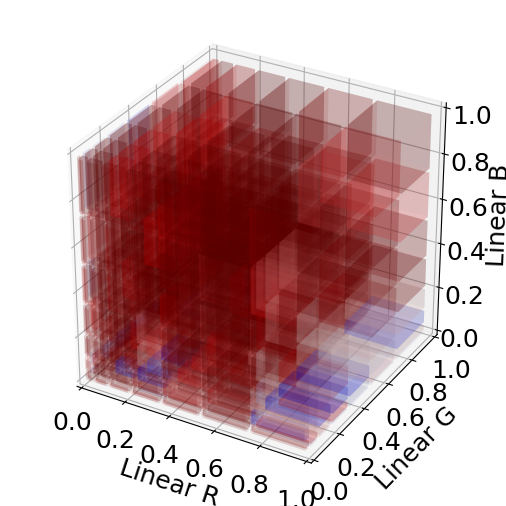
\includegraphics[width=\linewidth]{figure/002_Pixel2_error_cuve.png}
		\caption{Pixel 2}
	\end{subfigure}
	\hfill
	\begin{subfigure}[]{0.25\columnwidth}
		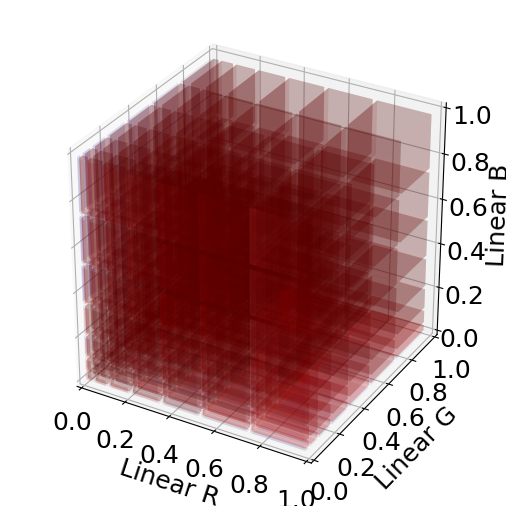
\includegraphics[width=\linewidth]{figure/003_MotoZ3_error_cuve.png}
		\caption{Moto Z3}
	\end{subfigure}
	\hfill
	\begin{subfigure}[]{0.25\columnwidth}
		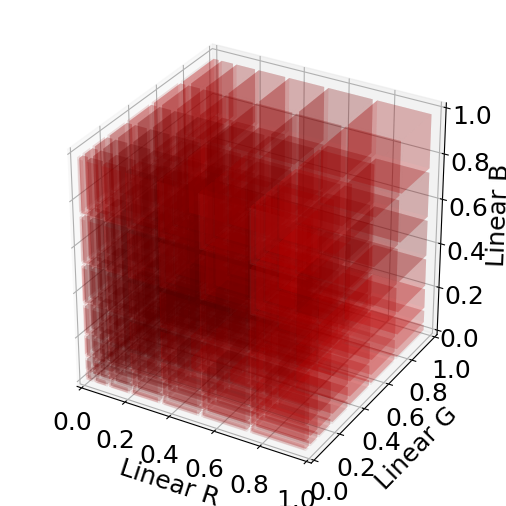
\includegraphics[width=\linewidth]{figure/004_Pixel4_error_cuve.png}
		\caption{Pixel 4}
	\end{subfigure}
	\hfill
	\begin{subfigure}[]{0.15\columnwidth}
		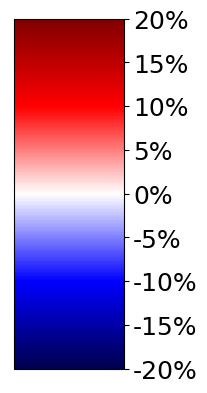
\includegraphics[width=0.8\linewidth]{figure/004_error_bar.png}
		% \caption{Error Bar}
	\end{subfigure}
        \vspace{-0.1in}
	\caption{Prediction error of the LMLR model in the linear RGB
          color space, for all sRGB values $(r, g, b)$, $r, g, b$
          are multiples of 16.}
        \vspace{-0.2in}
	\label{fig:error_wrt_linear}
\end{figure}


\paragraph{Model error across the color space.}
%  
% {what model did we use for this?}
Since prior-art models cannot even approximate 4 monochromatic
colors well, we can expect that they will have high prediction errors
in the entire 3-D color space. We further measured
the prediction error of the {LMLR} model at all RGB values of $(x, y,
z)$ where $x, y, z$ spans all multiples of 16. The results, shown
in Figure~\ref{fig:error_wrt_linear}, confirm that the {LMLR} model
exhibits high error across the color space on all three phones,
with a mean absolute prediction error of 6.90\%, 10.35\%, 7.10\%,
and 90th percentile absolute error of  15.65\%, 22.07\%, 16.19\%,
respectively, for the three phones.
Interestingly, the error is lower on Pixel 2 and Pixel 4, which can be explained
by their least violation of superposition property as shown in Figure~\ref{fig:initial_evaluation_2}.
Similarly, we observed that the {NLM} model also
exhibits high error across the color space on all three phones,
with a mean absolute prediction error of 6.79\%, 12.94\%, 6.02\%,
and 90th percentile absolute error of  15.45\%, 28.75\%, 13.38\%,
respectively, for the three phones.
% \comment{
% with a mean absolute prediction error of ???\%, ??\%, and ??\%,
% and 90th percentile absolute error of  ???\%, ??\%, and ??\%,
% respectively.
% }
% Interestingly, the error is lower on Pixel 2, which can be explained
% by its least violation of superposition property shown in Figure~\ref{fig:initial_evaluation_2}.

% \comment{can we add these error numbers for NLM?}
